\section{Interrupt Flag Register}
\begin{figure}[h!]
  
\includegraphics[width = 0.8\textwidth]{./figures/IFR.png}
  \caption{The flag register. (Courtesy of Intel Corporation.)}
\end{figure}
\begin{itemize}
  \item Clearing TF and IF ($2{nd}$ step in operation in Real mode)
  \item Set or clear IF: STI or CLI instructions
  \item Set or clear TF: No special instruction(Interrupt Service procedure)
\end{itemize}
\subsection{Enable Trap Flag}

\begin{lstlisting}
;A procedure that sets the TRAP flag bit to enable trapping

TRON PROC NEAR
  PUSH AX;
  PUSH BP

  MOV BP,SP ;Get SP
  MOV AX,[BP+8] ;Get flags
  OR AH,1 ; Set TF
  MOV [BP+8],AX ;Save flags

  POP BP ;Restore Reg
  POP AX
TRON ENDP
\end{lstlisting}
\subsection{Disable Trap Flag}

\begin{lstlisting}
;A procedure that sets the TRAP flag bit to enable trapping

TRON PROC NEAR
  PUSH AX;
  PUSH BP

  MOV BP,SP ;Get SP
  MOV AX,[BP+8] ;Get flags
  AND AH,0FEH ;Clear TF
  MOV [BP+8],AX ;Save flags

  POP BP ;Restore Reg
  POP AX
TRON ENDP
\end{lstlisting}

\section{Hardware Interrupts}

\textbf{NMI} : (+)ve edge triggered; After a positive edge , NMI must retain 1 until it is recognized by the microprocessor.
NMI is used for parity errors and other major system faults such as power failure.

\begin{figure}[h!]
  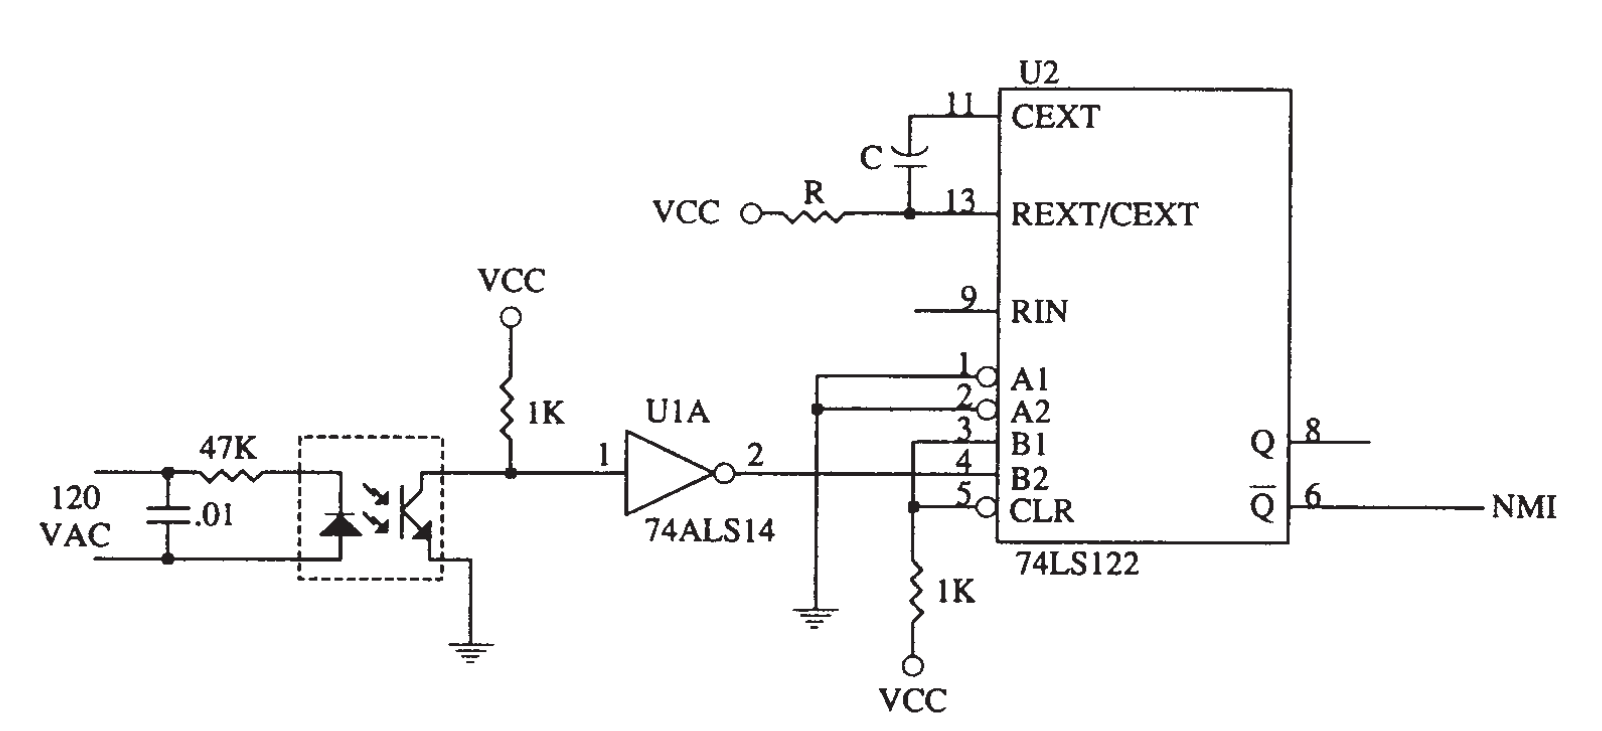
\includegraphics[width = 0.8\textwidth]{./figures/NMI.png}
  \caption{A power failure detection circuit.}
\end{figure}

\begin{itemize}
  \item An optical isolator provides isolation from the AC power lines
  \item Output of the isolator is shapped by a \textbf{Schmitt-trigger} inverter to feed to 74LS122 monostable multivibrator. As long as AC power is applied, Q remains at logic 1 having $\overline{Q}$ at 0.
  \item If power fails, 4LS122 no longer receives trigger pulse from 74ALS14. It makes $\overline{Q}$ to go 1 interrupting the $\mu P$ by NMI pin.
  \item It is assumed that the system power supply has a large enough filter capacitor to provide energy for at least 75 ms after the AC power ceases.
\end{itemize}
\subsection{INTR and $\overline{INTA}$}
\begin{itemize}
  \item INTR is level sensitive (must be held 1 until recognized)
  \item INTR is set by external event and cleared inside the interrupt service procedure
\end{itemize}

\begin{figure}[h!]
  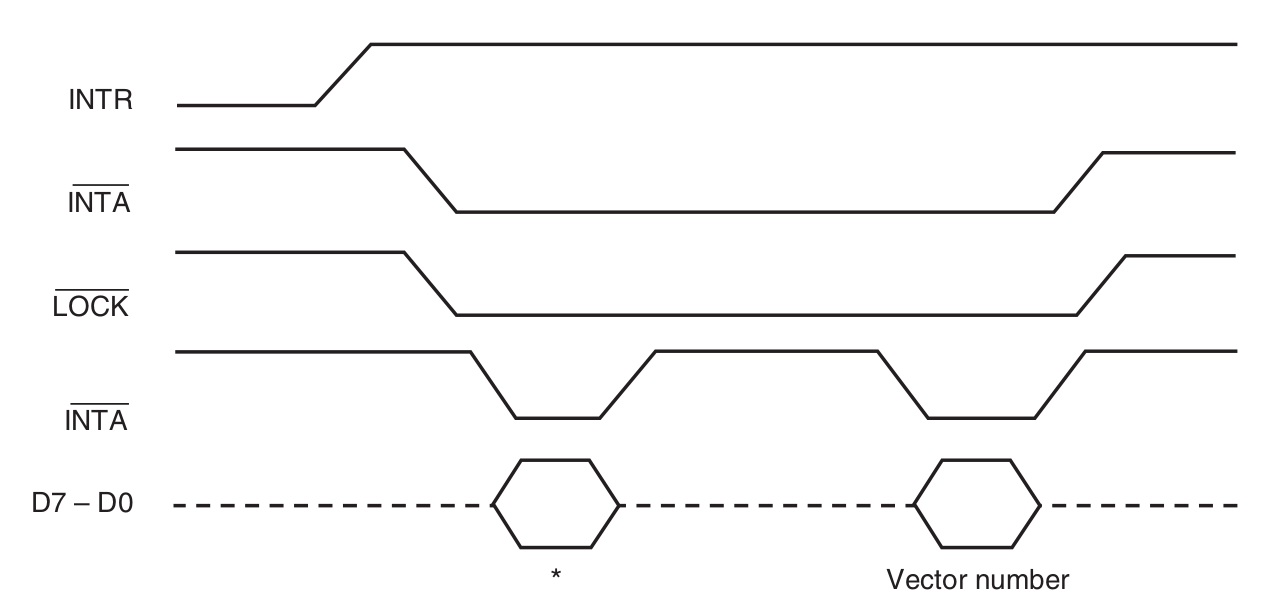
\includegraphics[width = 0.8\textwidth]{./figures/INTR_Timing.png}
  \caption{The timing of the INTR input and INTA output. *This portion of the data bus is ignored and usually contains the vector number.}
\end{figure}

\subsection{Making INTR input edge triggered}
\begin{figure}[h!]
  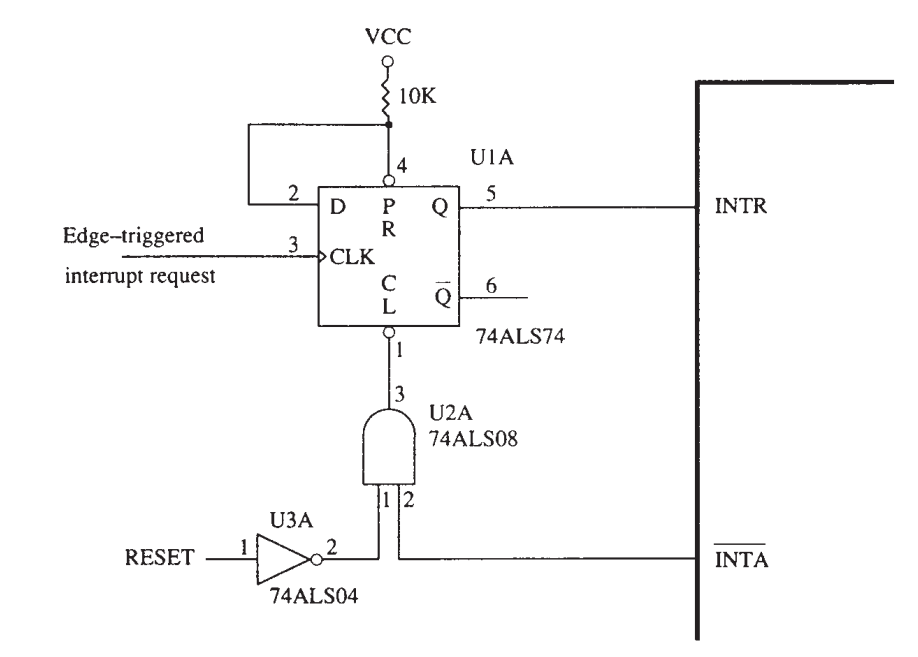
\includegraphics[width = 0.8\textwidth]{./figures/INTR_Edge.png}
  \caption{Converting INTR into an edge-triggered interrupt request input.}
\end{figure}

\subsection{Applying a fiex interrupt vector number FFH}
\begin{figure}[h!]
  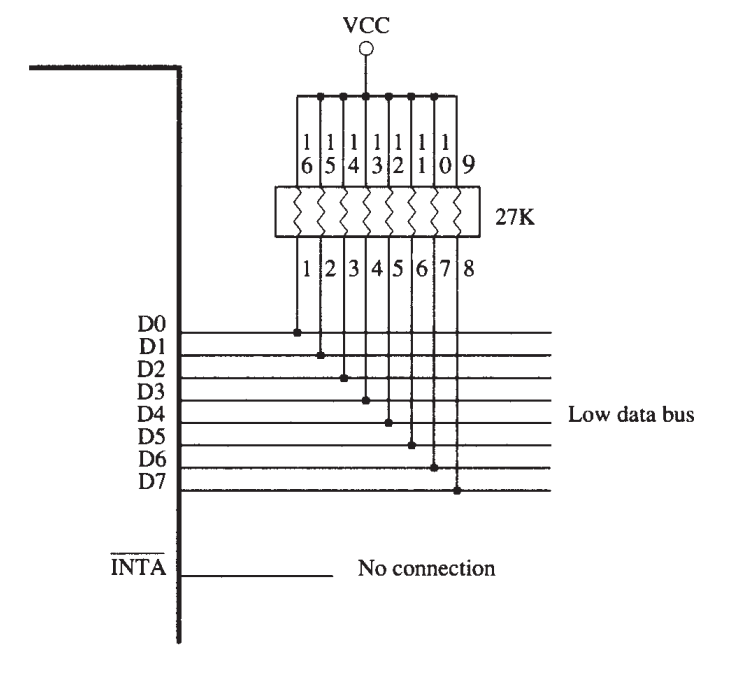
\includegraphics[width = 0.8\textwidth]{./figures/INTR_FFH.png}
  \caption{A simple method for generating interrupt vector type number FFH in response to INTR.}
\end{figure}

\subsection{Using a 3-state buffer to place a vector type number 80H}
\begin{figure}[h!]
  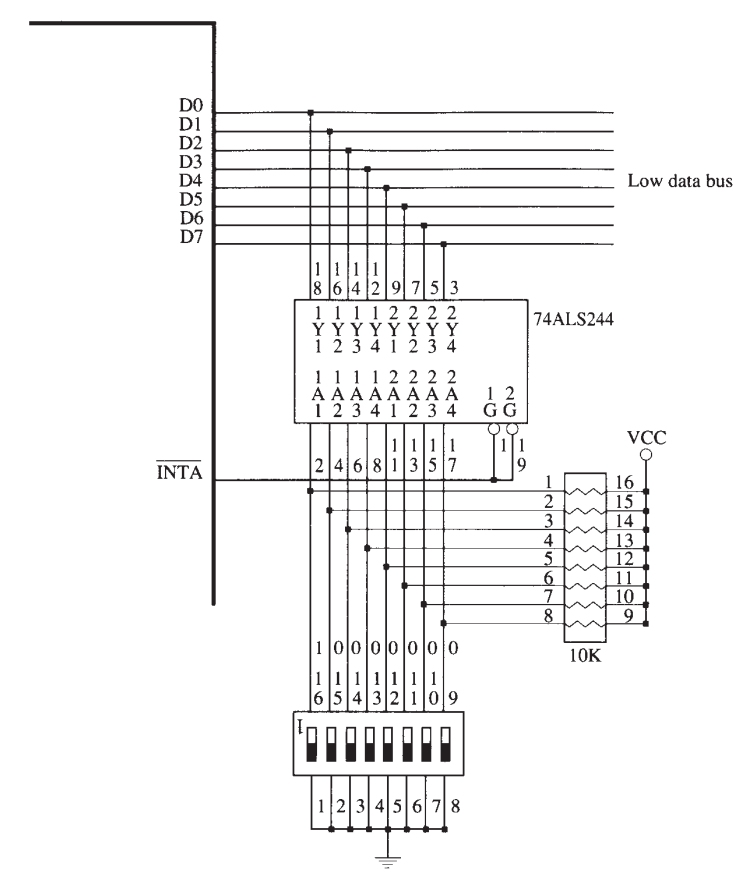
\includegraphics[width = 0.8\textwidth]{./figures/INTR_80H.png}
  \caption{A circuit that applies any interrupt vector type number in response to INTA . Here the circuit is applying type number 80H.}
\end{figure}

\subsection{Using 74ALS244 to expand to accomodate up to 7 interrupt inputs}
\begin{figure}[h!]
  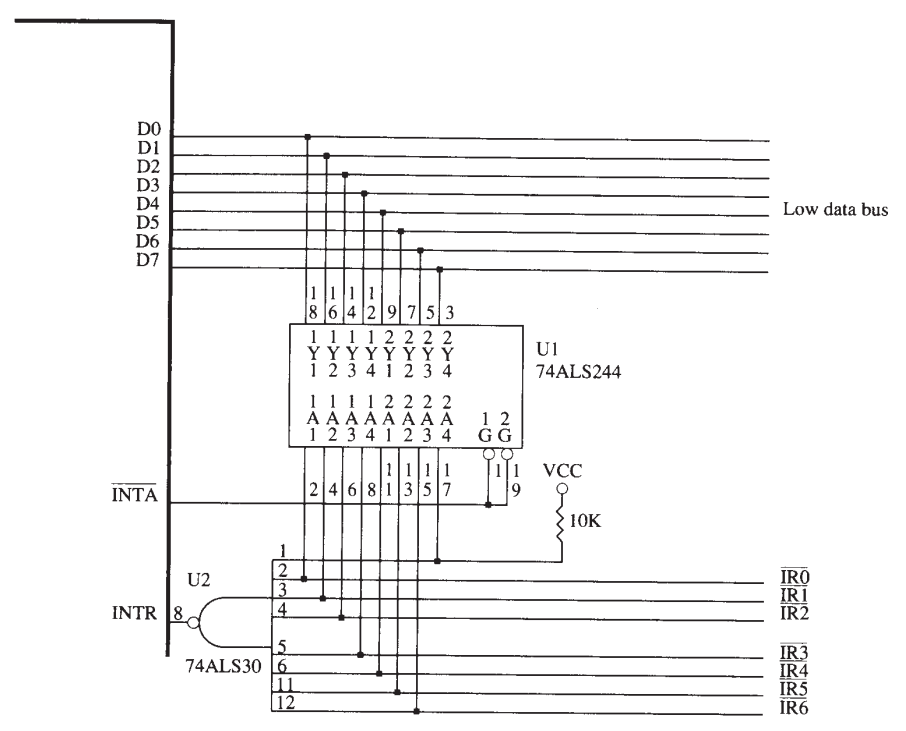
\includegraphics[width = 0.8\textwidth]{./figures/INTR_Expand.png}
  \caption{Expanding the INTR input from one to seven interrupt request lines.}
  \label{fig: INTR_Expand}
\end{figure}

\begin{figure}[h!]
  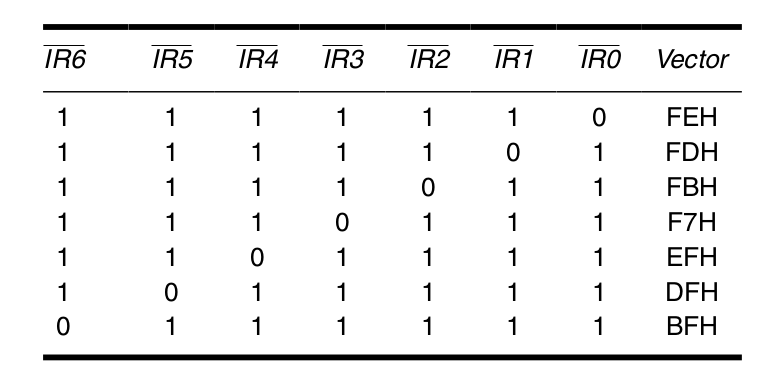
\includegraphics[width = 0.8\textwidth]{./figures/INTR_Table.png}
  \caption{Single interrupt requests for Figure \ref{fig: INTR_Expand}.}

\end{figure}

$2^7$ locations must be used which is wasteful. the solution is \textbf{Daisy-Chained Interrupts}

\subsection{Daisy-Chained Interrupts}
\begin{figure}[h!]
  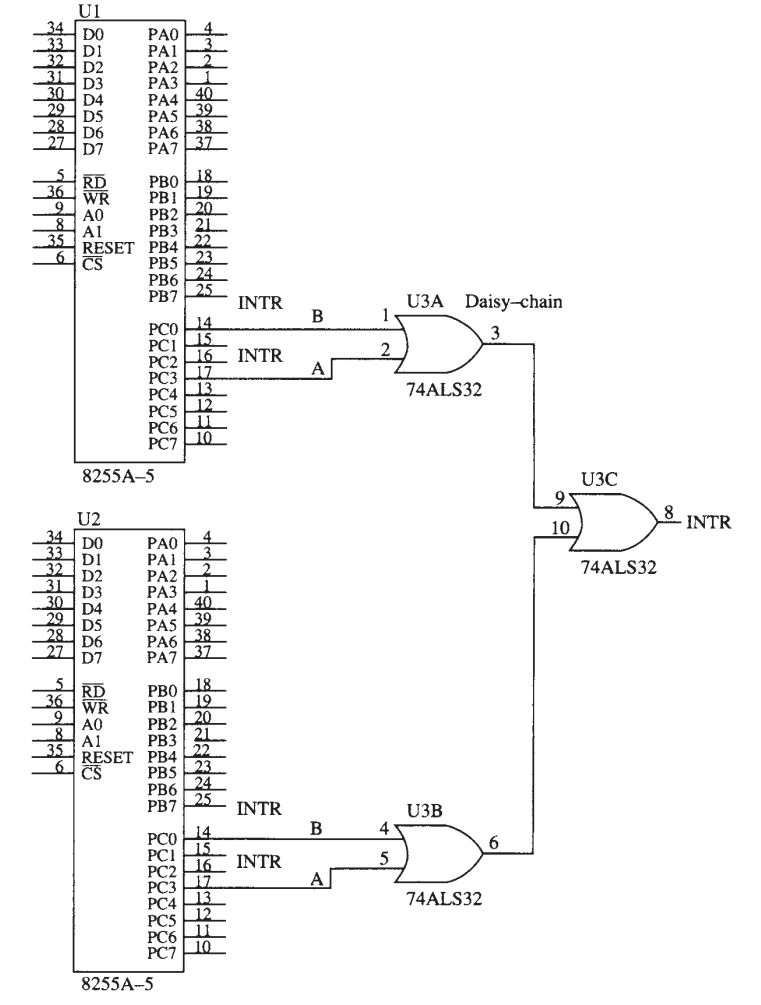
\includegraphics[width = 0.8\textwidth]{./figures/Daisy_Chain.png}
  \caption{Two 82C55 PIAs connected to the INTR outputs are daisy-chained to produce an INTR signal.}
  \label{fig: Daisy_Chain}
\end{figure}

\section{8259A programmable interrupt controller (PIC)}
\begin{itemize}
  \item Adds eight vectored priority encoder interrupts to the $\mu P$
  \item Can be expanded to accept 64 interrupt requents without additional hardware (One Master 259A , 8 slave 8259A)
  \item Pins of 259A
  \begin{enumerate}
    \item \textbf{IR7-IRO}: Interrupt requests
    \item \textbf{CAS2-CAS0}: Cascade lines
    \item $SP/\overline{EN}$: Slave program/ Enable buffer
    \item \textbf{A0}: Selects different command words.
  \end{enumerate}
  \item Command Words:
  \begin{enumerate}
    \item Initialization command words (ICW)
    \begin{itemize}
      \item \textbf{ICW1,ICW2}: Always
      \item \textbf{ICW3}: for cascading
      \item \textbf{ICW4}: for 8086 onward
    \end{itemize}
    \item Operation COmmand Words (OCW) :3
  \end{enumerate}
\end{itemize}

\textbf{Details of Command Word : ******SELF-STUDY*****}
